%% NOT DOCUMENTED YET:
%% MX, MY, MT, EX, EY, ET, E2, RESIDUUM, MAXSTEPSCO, MAXSTEPSSI, ORDERMAPS,
%% MAGSYM, CORRT, R, FLIPX, FLIPY, ROTATE90, ROTATE180, ROTATE270, NPDARKCUR,
%% INWARDMARGIN, EINITHR, FNA, FNB, FNY, FNVYZERO, FNYSECOND, FNPHIW, FNBETA,
%% FNFIELDTHR, FNMAXEMI, SECONDARYFLAG, NEMISSIONMODE, VSEYZERO, VEZERO,
%% VSEYMAX, VEMAX, VKENERGY, VKTHETA, VVTHERMAL, VW, SURFMATERIAL

\ifdefined \buildingFullOPALManual \else


%\ifx \@buildingFullOPALManual \@empty
%\else

%\documentclass[12pt,a4paper]{report}
\documentclass[a4paper]{book}

%% does not work in Latex2Html mode
%\usepackage{hyperref}

\usepackage[T1]{fontenc}
\usepackage{url}
\usepackage{html}
\usepackage{epic}
\usepackage{eepic}
\usepackage{makeidx}
\usepackage{array}
\usepackage{times}
\usepackage{amsmath}
\usepackage{amsxtra}
\usepackage{bm}
\usepackage[thin,thinp,thinc]{esdiff}
\usepackage{graphicx}
\usepackage{dingbat}
\usepackage{color}
\usepackage{subfig}
\usepackage{boxedminipage}
\usepackage{alltt}
\usepackage{nicefrac}
\usepackage{calc}
%\usepackage{pdfdraftcopy}             % Draft
\usepackage{tikz}
\usetikzlibrary{
  er,3d,calc,fadings,trees,positioning,arrows,chains,decorations.pathreplacing,
  decorations.pathmorphing,shapes,shapes.symbols,shapes.arrows,matrix,through,decorations.text
}

\tikzset{
  >=stealth',
  punktchain/.style={rectangle,rounded corners, draw=black, very thick,text width=10em,
                     minimum height=3em, text centered, on chain},
  line/.style={draw, thick, <-},
  element/.style={tape,top color=white,bottom color=blue!50!black!60!,minimum width=8em,
                  draw=blue!40!black!90, very thick,text width=10em, minimum height=3.5em,
                  text centered, on chain},
  every join/.style={->, thick,shorten >=1pt},
  tuborg/.style={decorate},
  tubnode/.style={midway, right=2pt}
}

\tikzstyle{material}=[draw, fill=blue!20, text width=16.0em, text centered, minimum height=1.5em]
\tikzstyle{diagramstep} = [material, text width=20em, minimum width=10em, minimum height=3em, rounded corners]
\tikzstyle{line} = [draw, thick, color=black!50, -latex']

\usepackage{booktabs}
\usepackage{xspace}
\usepackage{xstring}

\usepackage{fancyvrb}
\usepackage{rotating}
\usepackage{float}

\usepackage{tabularx}
\usepackage{longtable}
\setcounter{LTchunksize}{3}

\usepackage[section]{placeins}
\usepackage{MnSymbol}
\usepackage{microtype}
\usepackage{setspace}
\usepackage{dcolumn}

\usepackage[vmargin={3.0cm,3.0cm},
            hmargin={2.0cm,3.0cm}]{geometry}

\usepackage{upgreek}
\usepackage[binary-units=true]{siunitx}
\sisetup{exponent-product = \cdot,math-ohm=\Upomega,text-ohm=\ensuremath{\Upomega}}
\DeclareSIUnit{\clight}{c}
\DeclareSIUnit\gauss{Ga}

\usepackage{engord}
\usepackage{wasysym}
\DeclareSIUnit[number-unit-product = \,]{\permill}{\permil}

\usepackage{hyperref}
\hypersetup{
    pdftitle          = The OPAL Framework,
    pdfauthor         = {Andreas Adelmann, Achim Gsell, Valeria Rizzoglio, Christof Metzger-Kraus,
                         Yves Ineichen, Xiaoying Pang, Steve Russell, Chuan Wang, Jianjun Yang,
                         Suzanne Sheehy, Chris Rogers, Daniel Winklehner},
    pdfsubject        = User's Reference Manual,
    pdffitwindow      = true,               % page fit to window when opened
    pdfnewwindow      = true,               % links in new window
    colorlinks        = true,               % false: boxed links; true: colored links
    linkcolor         = black!80!green,     % color of internal links
    citecolor         = black!20!red,       % color of links to bibliography
    urlcolor          = blue,               % color of external links
    breaklinks        = true,
    bookmarksnumbered = true,
    plainpages        = false
}

\usepackage{ifthen}

\newif \iflinuxwindows
\linuxwindowstrue   % set this to true when building the manual on Linux or Windows
\iflinuxwindows
\usepackage{epstopdf}
\fi

\usepackage[backend=biber,
            style=phys,
            biblabel=brackets,
            maxnames=3,
            doi=true,
            isbn=true,
            url=true]{biblatex}
%---- macros ----

\renewcommand{\topfraction}{1.0}
\renewcommand{\bottomfraction}{1.0}
\renewcommand{\textfraction}{0.0}
\renewcommand{\arraystretch}{2.0}
\newenvironment{tex2html_nowrap}{}{}


\newcommand{\Newline}{\hfil \\}


\newsavebox{\ExampleBox}
\newenvironment{example}
 {\VerbatimEnvironment
  \begin{flushleft}
  \begin{lrbox}{\ExampleBox}
    \begin{minipage}{\linewidth}
  \begin{Verbatim}[frame=lines,xleftmargin=0cm,fontsize=\footnotesize,samepage=true]}
 {\end{Verbatim}
  \end{minipage}
  \end{lrbox}
  \mbox{\usebox{\ExampleBox}}
  \end{flushleft}
 }

\newenvironment{longexample}
{\Verbatim[frame=lines,xleftmargin=0mm,fontsize=\footnotesize]}
{\endVerbatim}

%\examplefromfile{filename} reads in a text file and displays it in the document.
\newcommand{\examplefromfile}[1]{
\VerbatimInput[frame=lines,xleftmargin=0mm,fontsize=\footnotesize,label=\texttt{#1}]{#1}}

%for upright d of differentials
\makeatletter
\newcount\my@repeat@count

\newcommand{\myrepeat}[2]{%
  \begingroup
  \my@repeat@count=\z@
  \@whilenum\my@repeat@count<#1\do{#2\advance\my@repeat@count\@ne}%
  \endgroup
}

\newcommand{\differential}[1]{\ifstrempty{#1}{\ES@dop\ES@difint}{\ES@dop^{#1}\ES@difint}}
\newcommand{\pdifferential}[1]{\ifstrempty{#1}{{\partial\,}}{{\partial^{#1}\,}}}

\makeatother

\newcommand{\der}[3][]{\frac{\differential{#1}#2}{\differential{}\ifstrempty{#1}{#3}{#3^#1}}}
\newcommand{\parder}[3][]{\frac{\pdifferential{#1}#2}{\pdifferential{}\ifstrempty{#1}{#3}{#3^#1}}}
\newcommand{\niceder}[3][]{\nicefrac{\differential{#1}#2}{\differential{}\ifstrempty{#1}{#3}{#3^#1}}}
\newcommand{\uglyder}[3][]{{\differential{#1}#2}/{\differential{}\ifstrempty{#1}{#3}{#3^#1}}}
\newcommand{\uglyparder}[3][]{{\pdifferential{#1}#2}/{\pdifferential{}\ifstrempty{#1}{#3}{#3^#1}}}
\newcommand{\dd}[1][]{\; \differential{#1}}
\newcommand{\primed}{^{\prime}}
\newcommand{\dprimed}{^{\prime\prime}}
\newcommand{\nprimed}[1]{^{\myrepeat{#1}{\prime}}}

%Editing Macros
\newcommand{\TODO}[1]{{\color{red}\ifthenelse{\boolean{ShowDebug}}{[TODO: #1]}{}}}



%text in gray box
\newsavebox{\fmbox}
\definecolor{lightgray}{gray}{0.95}
\newenvironment{fmpage}
   {\vspace{-1.0cm}\begin{lrbox}{\fmbox}\begin{minipage}[t]{13.5cm}\vspace{0.1cm}}
   {\vspace{-0.4cm}\end{minipage}\end{lrbox}\begin{center}\fcolorbox{black}{lightgray}{\usebox{\fmbox}}\end{center}}


% Definition new signes
\newcommand{\R}{{\mathbb R}} % real numbers
\newcommand{\Q}{{\mathbb Q}} % rational numbers
\newcommand{\Z}{{\mathbb Z}} % integer numbers
\newcommand{\N}{{\mathbb N}} % natural numbers

\newcommand{\mad}{\textsc{mad}\xspace}
\newcommand{\madnine}{\textsc{mad9}\xspace}
\newcommand{\madninep}{\textsc{mad9p}\xspace}
\newcommand{\madeight}{\textsc{mad8}\xspace}
\newcommand{\classic}{\textsc{classic}\xspace}

\makeatletter
\newcommand{\opal@impl}{\textsc{Opal}}
\newcommand{\opalt@impl}{\textsc{Opal-t}}
\newcommand{\opalcycl@impl}{\textsc{Opal-cycl}}
\newcommand{\opalmap@impl}{\textsc{Opal-map}}
\newcommand{\opalenv@impl}{\textsc{Opal-e}}

\newcommand{\opal}{\opal@impl\xspace}
\newcommand{\opalt}{\opalt@impl\xspace}
\newcommand{\opalcycl}{\opalcycl@impl\xspace}
\newcommand{\opalmap}{\opalmap@impl\xspace}
\newcommand{\opalenv}{\opalenv@impl\xspace}

\newcommand{\noopalt}{\leftthumbsdown \opalt@impl\xspace}
\newcommand{\noopalcycl}{\leftthumbsdown \opalcycl@impl\xspace}
\newcommand{\noopalmap}{\leftthumbsdown \opalmap@impl\xspace}
\newcommand{\noopalenv}{\leftthumbsdown \opalenv@impl\xspace}
\makeatother

\newcommand{\impactt}{\textsc{Impact-t}\xspace}
\newcommand{\partroot}{\textsc{H5root}}


\newcommand{\latermore}{More details will be given in Version 1.6.0}


\newcommand{\lieop}[1]{{:}{#1}{:}}

\newcommand{\rms}[1]{\overset{\sim}{#1}}

\newcommand{\sprod}{\cdot}
\newcommand{\vprod}{\times}
\newcommand{\matr}[1]{\mathcal{#1}}
\renewcommand{\vec}[1]{{\bm{#1}}}
\newcommand{\transpose}[1]{#1^\intercal}
\renewcommand{\epsilon}{\varepsilon}

\newcommand{\keyword}[2][]{\ifstrempty{#1}{\texttt{\expandafter\MakeUppercase\expandafter{#2}}}{\hyperref[#1]{\texttt{\expandafter\MakeUppercase\expandafter{#2}}}}}
\newcommand{\tabline}[3][]{\keyword[#1]{#2}& #3 \\}
\newcommand{\tabheadcell}[1]{{\bfseries #1}}

\newcommand*\kdescriptionlabel[1]{\hspace\labelsep
                                \normalfont\keyword{#1}\index{#1}}
\makeatletter
\newenvironment{kdescription}
               {\list{}{\labelwidth\z@ \itemindent-\leftmargin
                        \let\makelabel\kdescriptionlabel}}
               {\endlist}
\makeatother

\ExplSyntaxOn
\NewDocumentCommand{\tabhead}{ m }
 {
  \seq_set_split:Nnn \l_tmpa_seq { & } { #1 }
  \bfseries \seq_use:Nn \l_tmpa_seq { & \bfseries } \\
 }

\NewDocumentCommand \multrefImpl { O{ } m m m } {
  \ifnumgreater{\clist_count:n {#4}}{1}{
    \seq_set_from_clist:Nn \l_tmpa_seq { #4 }

    \seq_set_map:NNn \l_tmpb_seq \l_tmpa_seq { \exp_not:n { \ref{#3:##1} } }
    \ifstrempty{#1}{#2s}{#1}~\seq_use:Nnnn \l_tmpb_seq {\ and\ } {,\ } {,\ and\ }
  }{
    #2~\ref{#3:#4}
  }
}

\NewDocumentCommand \multeqnrefImpl { m } {
  \ifnumgreater{\clist_count:n {#1}}{1}{
    \seq_set_from_clist:Nn \l_tmpa_seq { #1 }

    \seq_set_map:NNn \l_tmpb_seq \l_tmpa_seq { \exp_not:n { \eqref{eq:##1} } }
    Equations~\seq_use:Nnnn \l_tmpb_seq {\ and\ } {,\ } {,\ and\ }
  }{
    Equation~\eqref{eq:#1}
  }
}
\ExplSyntaxOff


%Abbreviations for Equations, Figures, and Tables
%\newcommand{\Equation}[1]{Equation~\eqref{#1}}

\newcommand{\bibref}[2]{#1 \cite{bib:#2}}
\newcommand{\figref}[1]{\multrefImpl{Figure}{fig}{#1}}
\newcommand{\chpref}[1]{\multrefImpl{Chapter}{chp}{#1}}
\newcommand{\appref}[1]{\multrefImpl[Appendices]{Appendix}{chp}{#1}}
\newcommand{\secref}[1]{\multrefImpl{Section}{sec}{#1}}
\newcommand{\ssecref}[1]{\multrefImpl{Section}{ssec}{#1}}
\newcommand{\tabref}[1]{\multrefImpl{Table}{tab}{#1}}
\newcommand{\eqnref}[1]{\multeqnrefImpl{#1}}

\newcommand{\seefig}[1]{(see~\figref{#1})}
\newcommand{\seechp}[1]{(see~\chpref{#1})}
\newcommand{\seesec}[1]{(see~\secref{#1})}
\newcommand{\seessec}[1]{(see~\ssecref{#1})}
\newcommand{\seetab}[1]{(see~\tabref{#1})}
\newcommand{\seeeqn}[1]{(see~\eqnref{#1})}

\newcommand{\filename}[1]{\emph{#1}}


% Define distances for bordering
\newcommand{\blockdist}{1.3}
\newcommand{\edgedist}{1.5}
\newcommand{\diagramstep}[2]{node (p#1) [diagramstep] {#2}}


% place chapter title page on odd pages
\let\stdchapter\chapter
\makeatletter
\renewcommand*{\chapter}{\if@openright\cleardoublepage\else\clearpage\fi\stdchapter}

\makeatother

\IfFileExists{./version.tex}{%
  \newcommand{\opalversion}[1]{Version \ifstrempty{#1}{1.9.0}{#1}\xspace}
%
}%
{%
  \newcommand{\opalversion}[1]{\ifstrempty{#1}{current Version}{Version #1}\xspace}%
}
\newboolean{ShowMap}
\setboolean{ShowMap}{false}

\newboolean{ShowEnv}
\setboolean{ShowEnv}{false}

\newboolean{ShowDebug}
\setboolean{ShowDebug}{false}

%----Control Structures
\newboolean{FullOPALManual}
\setboolean{FullOPALManual}{false}


\makeindex


\bibliography{bibliography}
\begin{document}

\fi

\chapter{Distribution Command}
\label{chp:distribution}
\index{Distribution Command|(}

\begin{table}[!htb]
  \begin{center}\footnotesize
    \caption{Possible distribution types. Note that the \keyword{SURFACEEMISSION} and \keyword{SURFACERANDCREATE}
    distribution types will not be discussed in this chapter. Instead, refer to
    \chpref{femiss} on field emission for using these types.}
    \label{tab:disttypes}
    \begin{tabularx}{\textwidth-1cm}{|l|X|}
      \hline
      \tabhead{Distribution Type & Description}
      \hline
      \tabline[sec:fromfiledisttype]{FROMFILE}{Initial distribution read in from text file provided by user
      \seesec{fromfiledisttype}.}
      %\hline
      \tabline[sec:gaussdisttype]{GAUSS}{Initial distribution generated using Gaussian distribution(s)
      \seesec{gaussdisttype}.}
      %\hline
      \tabline[sec:flattopdisttype]{FLATTOP}{Initial distribution generated using flattop distribution(s)
      \seesec{flattopdisttype}.}
      %\hline
      \tabline[sec:binomialdisttype]{BINOMIAL}{Initial distribution generated using binomial distribution(s)
      \seesec{binomialdisttype}.}
      %\hline
      \tabline[chp:femiss]{SURFACEEMISSION}{For dark current and multipacting simulations. This type of distribution will not be covered in this chapter, see instead \chpref{femiss}. }
      %\hline
      \tabline[chp:femiss]{SURFACERANDCREATE}{For dark current and multipacting simulations. This type of distribution will not be covered in this chapter, see instead \chpref{femiss}. }
      %\hline
      \tabline[sec:gungaussflattopthdisttype]{GUNGAUSSFLATTOPTH}{Legacy. Special case of \keyword{FLATTOP} distribution \seesec{gungaussflattopthdisttype}.}
      %\hline
      \tabline[sec:astraflattopthdisttype]{ASTRAFLATTOPTH}{Legacy. Special case of \keyword{FLATTOP} distribution \seesec{astraflattopthdisttype}.}
      \hline
      \end{tabularx}
    \end{center}
\end{table}

The distribution command is used to introduce particles into an \opal simulation. Like other \opal
commands \seechp{format}, the distribution command is of the form:

\begin{example}
Name:DISTRIBUTION, DISTRIBUTION = TYPE,
                   ATTRIBUTE #1 =,
                   ATTRIBUTE #2 =,
                   .
                   .
                   .
                   ATTRIBUTE #N =;
\end{example}
The distribution is given a name (which is used to reference the distribution in the \opal input
file), a distribution type, and a list of attributes. The types of distributions that are supported
are listed in \tabref{disttypes}. The attributes that follow the distribution type further
define the particle distribution. Some attributes are universal, while others are specific to the
distribution type. In the following sections we will define the distribution attributes, starting
with the general, or universal attributes. (Note that, in general, if a distribution type does not
support a particular attribute, defining a value for it does no harm. That attribute just gets ignored.)

\section{Units}
\label{sec:unitsdistattributes}
\index{Distribution!Units}
\FloatBarrier

The internal units used by \opalt and \opalcycl are described in \secref{variablesopalt,variablesopalcycl}.
When defining a distribution, both \opalt and \opalcycl use meters for
length and seconds for time. However, there are different options for the units used to input the
momentum. This is controlled with the \keyword{INPUTMOUNITS} attribute, defined in
\tabref{distattrinputmounits}.

\begin{table}[!htb]
  \begin{center}\footnotesize
    \caption{Definition of \keyword{INPUTMOUNITS} attribute.}
    \label{tab:distattrinputmounits}
    \begin{tabularx}{\textwidth-1cm}{|l|c|X|}
      \hline
      \tabhead{Attribute Name & Value & Description}
      \hline
      \tabline[sec:variablesopalt]{INPUTMOUNITS}{\keyword{NONE} (default for \opalt) & Use no units for the input momentum (e.g. $p_{x}$, $p_{y}$, $p_{z}$). Momentum is given as $\beta_{x} \gamma$, $\beta_{y} \gamma$ and $\beta_{z} \gamma$, as in \secref{variablesopalt}.}
      \tabline{INPUTMOUNITS}{\index{INPUTMOUNITS} \keyword{EV} (default for \opalcycl) & Use the units \si{\electronvolt} for the input momentum (e.g. $p_{x}$, $p_{y}$, $p_{z}$).}
      \hline
    \end{tabularx}
  \end{center}
\end{table}

\section{General Distribution Attributes}
\label{sec:gendistattributes}
\index{Distribution!General Attributes}
\FloatBarrier

Once the distribution type is chosen, the next attribute to specify is the \keyword{EMITTED}
attribute, which is defined in \tabref{distattremitted}. The \keyword{EMITTED} attribute
controls whether a distribution is \emph{injected} or \emph{emitted}. An \emph{injected} distribution
is placed in its entirety into the simulation space at the start of the simulation. An
\emph{emitted} beam is emitted into the simulation over time as the simulation progresses (e.g.
from a cathode in a photoinjector simulation). Currently, only \opalt supports \emph{emitted}
distributions. The default is an \emph{injected} distribution.

\begin{table}[!htb]
  \begin{center}\footnotesize
    \caption{Definition of \keyword{EMITTED} attribute.}
    \label{tab:distattremitted}
    \begin{tabularx}{\textwidth-1cm}{|l|c|X|}
      \hline
      \tabhead{Attribute Name & Value & Description }
      \hline
      \tabline{EMITTED}{\index{EMITTED} \keyword{FALSE} (default)   & The distribution is injected into the simulation in its entirety
      at the start of the simulation. The particle coordinates for an injected distribution are defined as in
      \secref{variablesopalt,variablesopalcycl}. Note that in \opalt the entire distribution will automatically
      be shifted to ensure that the $z$ coordinate will be greater than zero for all particles.}
      %\hline
      \tabline[sec:variablesopalt]{EMITTED}{\keyword{TRUE} & The distribution is emitted into the simulation over time as the simulation
      progresses. Currently only \opalt supports this type of distribution. In this case, the longitudinal coordinate, as
      defined by \secref{variablesopalt}, is given in seconds instead of meters. Early times are emitted first.}
      \hline
    \end{tabularx}
  \end{center}
\end{table}

Depending on the \keyword{EMITTED} attribute, we can specify several other attributes that do not depend on the
distribution type. These are defined in \secref{universaldistattributes,injecteddistattributes,emitteddistattributes} in
\tabref{distattruniversal,distattrinjected,distattrsemitted}.
\clearpage
\subsection{Universal Attributes}
\label{sec:universaldistattributes}
\index{Distribution!Universal Attributes}
\begin{table}[!htb]
  \begin{center}\footnotesize
    \caption{Definition of universal distribution attributes. Any distribution type can use these
      and they are the same whether the beam is \emph{injected} or \emph{emitted}.}
    \label{tab:distattruniversal}
    \begin{tabularx}{\textwidth-1cm}{|l|c|c|X|}
      \hline
      \tabhead{Attribute Name & Default Value & Units & Description }
      \hline
      \tabline{WRITETOFILE}{\index{WRITETOFILE} \keyword{FALSE} & None & Echo initial distribution to text file \filename{data/distribution.data}.}
      %\hline
      \tabline[sec:distlist]{WEIGHT}{\num{1.0} & None & Weight of distribution when used in a distribution list \seesec{distlist}.}
      %\hline
      \tabline[sec:FSENBINS]{NBIN}{\num{0} & None & The distribution (beam) will be broken up into \keyword{NBIN} energy bins.
      This has consequences for the space charge solver \seesec{FSENBINS}.}
      %\hline
      \tabline{XMULT}{\index{XMULT} \num{1.0} & None & Value used to scale the $x$ positions of the distribution
      particles. Applied after the distribution is generated (or read in).}
      %\hline
      \tabline{YMULT}{\index{YMULT} \num{1.0} & None & Value used to scale the $y$ positions of the distribution
      particles. Applied after the distribution is generated (or read in).}
      %\hline
      \tabline{PXMULT}{\index{PXMULT} \num{1.0} & None & Value used to scale the x momentum, $p_{x}$, of the
      distribution particles. Applied after the distribution is generated (or read in).}
      %\hline
      \tabline{PYMULT}{\index{PYMULT} \num{1.0} & None & Value used to scale the y momentum, $p_{y}$, of the
      distribution particles. Applied after the distribution is generated (or read in).}
      %\hline
      \tabline{PZMULT}{\index{PZMULT} \num{1.0} & None & Value use to scale the z momentum, $p_{z}$, of the
      distribution particles. Applied after the distribution is generated (or read in).}
      %\hline
      \tabline{OFFSETX}{\index{OFFSETX} \num{0.0} & \si{\meter} & Distribution is shifted in $x$ by this amount after the distribution
      is generated (or read in). Same as the average $x$ position, $\bar{x}$.}
      %\hline
      \tabline{OFFSETY}{\index{OFFSETY} \num{0.0} & \si{\meter} & Distribution is shifted in $y$ by this amount after the distribution
      is generated (or read in). Same as the average $y$ position, $\bar{y}$.}
      %\hline
      \tabline{OFFSETPX}{\index{OFFSETPX} \num{0.0} & \secref{unitsdistattributes} &
      Distribution is shifted in $p_{x}$ by this amount after the distribution is generated (or read in). Same as the
      average $p_{x}$ value, $\bar{p}_{x}$.}
      %\hline
      \tabline{OFFSETPY}{\index{OFFSETPY} \num{0.0} & \secref{unitsdistattributes} &
      Distribution is shifted in $p_{y}$ by this amount after the distribution is generated (or read in). Same as the
      average $p_{y}$ value, $\bar{p}_{y}$.}
      %\hline
      \tabline{OFFSETPZ}{\index{OFFSETPZ} \num{0.0} & \secref{unitsdistattributes} &
      Distribution is shifted in $p_{z}$ by this amount after the distribution is generated (or read in). Same as the
      average $p_{z}$ value, $\bar{p}_{z}$.}
      \hline
    \end{tabularx}
  \end{center}
\end{table}

\subsection{Injected Distribution Attributes}
\label{sec:injecteddistattributes}
\index{Distribution!Injected Beam}
\begin{table}[!htb]
  \begin{center}\footnotesize
    \caption{Definition of distribution attributes that only affect \emph{injected} beams.}
    \label{tab:distattrinjected}
    \begin{tabularx}{\textwidth-1cm}{|l|c|c|X|}
      \hline
      \tabhead{Attribute Name & Default Value & Units & Description }
      \hline
      \tabline{ZMULT}{\index{ZMULT} \num{1.0} & None & Value used to scale the $z$ positions of the distribution
      particles. Applied after the distribution is generated (or read in).}
      %\hline
      \tabline{OFFSETZ}{\index{OFFSETZ} \num{0.0} & \si{\meter} & Distribution is shifted in $z$ by this amount relative to the reference particle. Same as the average $z$ position, $\bar{z}$.}
      \hline
    \end{tabularx}
  \end{center}
\end{table}

\subsection{Emitted Distribution Attributes}
\label{sec:emitteddistattributes}
\index{Distribution!Emitted Beam}
\begin{table}[!htb]
  \begin{center}\footnotesize
    \caption{Definition of distribution attributes that only affect \emph{emitted} beams.}
    \label{tab:distattrsemitted}
    \begin{tabularx}{\textwidth-1cm}{|l|c|c|X|}
      \hline
      \tabhead{Attribute Name  & Default Value & Units & Description }
      \hline
      \tabline{TMULT}{\index{TMULT} \num{1.0} & None & Value used to scale the $t$ values of the distribution
      particles. Applied after the distribution is generated (or read in).}
      %\hline
      \tabline{OFFSETT}{\index{OFFSETT} \num{0.0} & \si{\second} & Distribution is emitted later by this amount relative to the reference particle.}
      %\hline
      \tabline{EMISSIONSTEPS}{\index{EMISSIONSTEPS}  \num{1} & None & Number of time steps to take during emission. The simulation time step
      will be adjusted during emission to ensure that this many time steps will be
      required to emit the entire distribution.}
      %\hline
      \tabline{EMISSIONMODEL}{\index{EMISSIONMODEL}  None & None & Emission model to use when emitting particles from cathode
      \seesec{emissionmodel}.}
      \hline
    \end{tabularx}
  \end{center}
\end{table}

\section{\keywordinheader{FROMFILE} Distribution Type}
\label{sec:fromfiledisttype}
\index{Distribution!FROMFILE}
\FloatBarrier

The most versatile distribution type is to use a user generated text file as input to \opal. This
allows the user to generate their own distribution, if the built in options in \opal are insufficient,
and have it either \emph{injected} or \emph{emitted} into the simulation. In \tabref{distattrfromfile}
we list the single attribute specific to this type of distribution type.

\begin{table}[!htb]
  \begin{center}\footnotesize
    \caption{Definition of distribution attributes for a \keyword{FROMFILE} distribution type.}
    \label{tab:distattrfromfile}
    \begin{tabularx}{\textwidth-1cm}{|l|c|c|X|}
      \hline
      \tabhead{Attribute Name & Default Value & Units & Description }
      \hline
      \tabline{FNAME}{\index{FNAME} None  & None & File name for text file containing distribution particle coordinates.}
      \hline
    \end{tabularx}
  \end{center}
\end{table}

An example of an \emph{injected} \keyword{FROMFILE} distribution definition is:

\begin{example}
Name:DISTRIBUTION, DISTRIBUTION = FROMFILE,
                   FNAME = ``text file name'';
\end{example}
an example of an \emph{emitted} \keyword{FROMFILE} distribution definition is:

\begin{example}
Name:DISTRIBUTION, DISTRIBUTION = FROMFILE,
                   FNAME = ``text file name'',
                   EMITTED = TRUE,
                   EMISSIONMODEL = None;
\end{example}

The text input file for the \keyword{FROMFILE} distribution type has slightly a slightly different
format, depending on whether the distribution is to be \emph{injected} or \emph{emitted}. The
\emph{injected} file format is defined in \tabref{fromfileinjfileformat}. The \emph{emitted}
file format is defined in \tabref{fromfileemitfileformat}.

\begin{table}[!htb]
  \begin{center}\footnotesize
    \caption{File format for \emph{injected} \keyword{FROMFILE} distribution type. N is the number
    of particles in the file. The particle coordinates are defined in \secref{variablesopalt,variablesopalcycl}.}
    \label{tab:fromfileinjfileformat}
    \begin{tabular}{llllll}
      \hline
      N & & & & & \\
      $x_{1}$ & $p_{x1}$ & $y_{1}$ & $p_{y1}$ & $z_{1}$ & $p_{z1}$ \\
      $x_{2}$ & $p_{x2}$ & $y_{2}$ & $p_{y2}$ & $z_{2}$ & $p_{z2}$ \\
      . & & & & & \\
      . & & & & & \\
      $x_{N}$ & $p_{xN}$ & $y_{N}$ & $p_{yN}$ & $z_{N}$ & $p_{zN}$ \\
      \hline
    \end{tabular}
  \end{center}
\end{table}

\begin{table}[!htb]
  \begin{center}\footnotesize
    \caption{File format for \emph{emitted} \keyword{FROMFILE} distribution type. N is the number
    of particles in the file. The particle coordinates are defined in \secref{variablesopalt}
    except that $z$, in meters, is replaced by $t$ in seconds.}
    \label{tab:fromfileemitfileformat}
    \begin{tabular}{llllll}
      \hline
      N & & & & & \\
      $x_{1}$ & $p_{x1}$ & $y_{1}$ & $p_{y1}$ & $t_{1}$ & $p_{z1}$ \\
      $x_{2}$ & $p_{x2}$ & $y_{2}$ & $p_{y2}$ & $t_{2}$ & $p_{z2}$ \\
      . & & & & & \\
      . & & & & & \\
      $x_{N}$ & $p_{xN}$ & $y_{N}$ & $p_{yN}$ & $t_{N}$ & $p_{zN}$ \\
      \hline
    \end{tabular}
  \end{center}
\end{table}

Note that for an \emph{emitted} \keyword{FROMFILE} distribution, all of the particle's time, $t$, coordinates
will be shifted to negative time (if they are not there already). The simulation clock will then start at $t = 0$
and distribution particles will be emitted into the simulation as the simulation progresses. Also note that,
as the particles are emitted, they will be modified according to the type of emission model used. This is defined
by the attribute \keyword{EMISSIONMODEL}, which is described in \secref{emissionmodel}. A choice of
\keyword{NONE} for the \keyword{EMISSIONMODEL} (which is the default) can be defined so as not to affect the
distribution coordinates at all.


To maintain consistency $N$ and \keyword{NPART} from the \keyword{BEAM} command in \chpref{beam} must be equal.

\section{\keywordinheader{GAUSS} Distribution Type}
\label{sec:gaussdisttype}
\index{Distribution!GAUSS|(}
\FloatBarrier

As the name implies, the \keyword{GAUSS} distribution type can generate distributions with a general
Gaussian shape (here we show a one-dimensional example):

\begin{equation*}
  f(x) = \frac{1}{\sqrt{2 \pi}} e^{-\frac{(x - \bar{x})^{2}}{2 \sigma_{x}^{2}}}
\end{equation*}
where $\bar{x}$ is the average value of $x$. However, the \keyword{GAUSS} distribution can also be used to
generate an emitted beam with a flat top time profile. We will go over the various options for the \keyword{GAUSS}
distribution type in this section.

\subsection{Simple \keywordinheader{GAUSS} Distribution Type}
We will begin by describing how to create a simple \keyword{GAUSS} distribution type. That is, a simple
6-dimensional distribution with a Gaussian distribution in all dimensions.

\begin{table}[!htb]
  \begin{center}\footnotesize
    \caption{Definition of the basic distribution attributes for a \keyword{GAUSS} distribution type.}
    \label{tab:distattrgauss}
    \begin{tabularx}{\textwidth-1cm}{|l|c|c|X|}
      \hline
      \tabhead{Attribute Name & Default Value & Units & Description }
      \hline
      \tabline{SIGMAX}{\index{SIGMAX}  \num{0.0}  & \si{\meter} & RMS width, $\sigma_{x}$, in transverse $x$ direction.}
      %\hline
      \tabline{SIGMAY}{\index{SIGMAY}  \num{0.0}  & \si{\meter} & RMS width, $\sigma_{y}$, in transverse $y$ direction.}
      %\hline
      \tabline{SIGMAR}{\index{SIGMAR}  \num{0.0} & \si{\meter} & RMS radius, $\sigma_{r}$, in radial direction. If nonzero \keyword{SIGMAR} overrides
      \keyword{SIGMAX} and \keyword{SIGMAY}.}
      %\hline
      \tabline{SIGMAZ}{\index{SIGMAZ}  \num{0.0}  & \si{\meter} & RMS length, $\sigma_{z}$, in longitudinal (z) direction. \keyword{SIGMAZ} is used
      for an \emph{injected} distribution.}
      %\hline
      \tabline{SIGMAT}{\index{SIGMAT}  \num{0.0}  & \si{\second} & RMS width, $\sigma_{t}$, in time (t). \keyword{SIGMAT} is used for an \emph{emitted}
      distribution.}
      %\hline
      \tabline{SIGMAPX}{\index{SIGMAPX}  \num{0.0} & \secref{unitsdistattributes}& Parameter $\sigma_{px}$ for defining distribution. }
      %\hline
      \tabline{SIGMAPY}{\index{SIGMAPY}  \num{0.0} & \secref{unitsdistattributes}& Parameter $\sigma_{py}$ for defining distribution. }
      %\hline
      \tabline{SIGMAPZ}{\index{SIGMAPZ}  \num{0.0} & \secref{unitsdistattributes}& Parameter $\sigma_{pz}$ for defining distribution. }
      %\hline
      \tabline{CUTOFFX}{\index{CUTOFFX} \num{3.0} & None & Defines transverse distribution cutoff in the $x$ direction in units of
      $\sigma_{x}$. If \keyword{CUTOFFX} $= 0$ then actual cutoff in $x$ is set to infinity.}
      %\hline
      \tabline{CUTOFFY}{\index{CUTOFFY} \num{3.0} & None & Defines transverse distribution cutoff in the $y$ direction in units of
      $\sigma_{y}$. If \keyword{CUTOFFY} $= 0$ then actual cutoff in $y$ is set to infinity.}
      %\hline
      \tabline{CUTOFFR}{\index{CUTOFFR} \num{3.0} & None & Defines transverse distribution cutoff in the $r$ direction in units of
      $\sigma_{r}$. If \keyword{CUTOFFR} $= 0$ then actual cutoff in $r$ is set to infinity. \keyword{CUTOFFR} is
      only used if \keyword{SIGMAR} $>0$.}
      %\hline
      \tabline{CUTOFFLONG}{\index{CUTOFFLONG}  \num{3.0} & None & Defines longitudinal distribution cutoff in the $z$ or $t$ direction
      (\emph{injected} or \emph{emitted}) in units of $\sigma_{z}$ or $\sigma_{t}$. \keyword{CUTOFFLONG} is
      different from other dimensions in that a value of \num{0.0} does not imply a cutoff value of infinity.}
      %\hline
      \tabline{CUTOFFPX}{\index{CUTOFFPX} \num{3.0} & None & Defines cutoff in $p_{x}$ dimension in units of $\sigma_{px}$.
      If \keyword{CUTOFFPX} $= 0$ then actual cutoff in $p_{x}$ is set to infinity.}
      %\hline
      \tabline{CUTOFFPY}{\index{CUTOFFPY} \num{3.0} & None & Defines cutoff in $p_{y}$ dimension in units of $\sigma_{py}$.
      If \keyword{CUTOFFPY} $= 0$ then actual cutoff in $p_{y}$ is set to infinity.}
      %\hline
      \tabline{CUTOFFPZ}{\index{CUTOFFPZ} \num{3.0} & None & Defines cutoff in $p_{z}$ dimension in units of $\sigma_{pz}$.
      If \keyword{CUTOFFPZ} $= 0$ then actual cutoff is $p_{z}$ is set to infinity.}
      \hline
    \end{tabularx}
  \end{center}
\end{table}

In \tabref{distattrgauss} we list the basic attributes available for a \keyword{GAUSS} distribution. We
can use these to create a very simple \keyword{GAUSS} distribution:

\begin{example}
Name:DISTRIBUTION, DISTRIBUTION = GAUSS,
                   SIGMAX = 0.001,
                   SIGMAY = 0.003,
                   SIGMAZ = 0.002,
                   SIGMAPX = 0.0,
                   SIGMAPY = 0.0,
                   SIGMAPZ = 0.0,
                   CUTOFFX = 2.0,
                   CUTOFFY = 2.0,
                   CUTOFFLONG = 4.0,
                   OFFSETX = 0.001,
                   OFFSETY = -0.002,
                   OFFSETZ = 0.01,
                   OFFSETPZ = 1200.0
                   USEEV = TRUE;
\end{example}
This creates a Gaussian shaped distribution with zero transverse emittance, zero energy spread, $\sigma_{x} = \SI{1.0}{\milli\meter}$,
$\sigma_{y} = \SI{3.0}{\milli\meter}$, $\sigma_{z} = \SI{2.0}{\milli\meter}$ and an average energy of:

\begin{equation*}
W = \SI{1.2}{\mega\electronvolt}
\end{equation*}
In the $x$ direction, the Gaussian distribution is cutoff at $x = 2.0 \times \sigma_{x} = \SI{2.0}{\milli\meter}$. In the $y$
direction it is cutoff at $y = 2.0 \times \sigma_{y} = \SI{6.0}{\milli\meter}$. This distribution is \emph{injected} into the simulation
at an average position of $(\bar{x},\bar{y},\bar{z})=(\SI{1.0}{\milli\meter}, \SI{-2.0}{\milli\meter}, \SI{10.0}{\milli\meter})$.



\subsection{\keywordinheader{GAUSS} Distribution for Photoinjector}
\label{sec:gaussdisttypephotoinjector}

\begin{table}[!htb]
  \begin{center}\footnotesize
    \caption{Definition of additional distribution attributes for an \emph{emitted} \keyword{GAUSS}
      distribution type. These are used to generate a distribution with a time profile as illustrated
      in \figref{flattop}.}
    \label{tab:distattremittedgauss}
    \begin{tabularx}{\textwidth-1cm}{|l|c|c|X|}
      \hline
      \tabhead{Attribute Name & Default Value & Units & Description }
      \hline
      \tabline{TPULSEFWHM}{\index{TPULSEFWHM}  \num{0.0}  & \si{\second} & Flat top time \seefig{flattop}. }
      %\hline
      \tabline{TRISE}{\index{TRISE} \num{0.0}  & \si{\second} & Rise time \seefig{flattop}. If defined will override
      \keyword{SIGMAT}.}
      %\hline
      \tabline{TFALL}{\index{TFALL} \num{0.0}  & \si{\second} & Fall time \seefig{flattop}. If defined will override
      \keyword{SIGMAT}.}
      %\hline
      \tabline{FTOSCAMPLITUDE}{\index{FTOSCAMPLITUDE} \num{0}  & None & Sinusoidal oscillations can imposed on the flat top in \figref{flattop}.
      This defines the amplitude of those oscillations in percent of the average flat top amplitude.}
      %\hline
      \tabline{FTOSCPERIODS}{\index{FTOSCPERIODS} \num{0} & None & Defines the number of oscillation periods imposed on the flat top,
      $t_\mathrm{flattop}$, in \figref{flattop}.}
      \hline
    \end{tabularx}
  \end{center}
\end{table}

\begin{figure}[ht]
  \begin{center}
    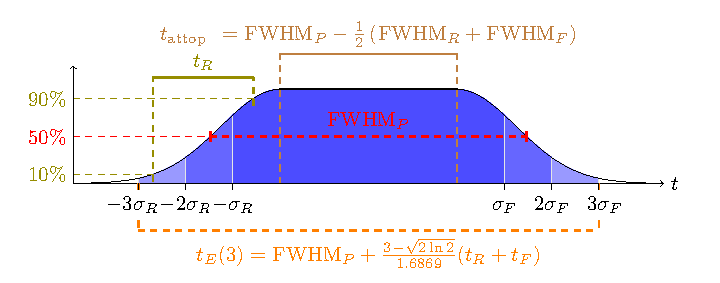
\includegraphics[width=0.8\textwidth]{./figures/flattop.pdf}
    \caption{\opal emitted \keyword{GAUSS} distribution with flat top.}
    \label{fig:flattop}
  \end{center}
\end{figure}

A useful feature of the \keyword{GAUSS} distribution type is the ability to mimic the initial distribution
from a photoinjector. For this purpose we have the distribution attributes listed in \tabref{distattremittedgauss}.
Using them, we can create a distribution with the time structure
shown in \figref{flattop}. This is a half Gaussian rise plus a uniform flat-top plus a half Gaussian
fall. To make it more convenient to mimic measured laser profiles, \keyword{TRISE} and \keyword{TFALL} from
\tabref{distattremittedgauss} do not define RMS quantities, but instead are given by (See also \figref{flattop}):

\begin{align*}
  \keyword{TRISE} = t_{R} &= \left(\sqrt{2 \ln(10)} - \sqrt{2 \ln \left(\frac{10}{9} \right)} \right) \sigma_{R}\\
  & = 1.6869 \sigma_{R} \\
  \keyword{TFALL} = t_{F} &= \left(\sqrt{2 \ln(10)} - \sqrt{2 \ln \left(\frac{10}{9} \right)} \right) \sigma_{F}\\
  & = 1.6869 \sigma_{F}
\end{align*}
where $\sigma_{R}$ and $\sigma_{F}$ are the Gaussian, RMS rise and fall times respectively. The flat-top portion
of the profile, \keyword{TPULSEFWHM}, is defined as (See also \figref{flattop}):

\begin{equation*}
  \keyword{TPULSEFWHM} = \mathrm{FWHM}_{P} = t_\mathrm{flattop} + \sqrt{2 \ln 2} \left( \sigma_{R} + \sigma_{F} \right)
\end{equation*}
Total emission time, $t_{E}$, of this distribution, is a function of the longitudinal cutoff,
\keyword{CUTOFFLONG} \seetab{distattrgauss}, and is given by:

\begin{align*}
  t_{E}(\keyword{CUTOFFLONG}) &= \mathrm{FWHM}_{P} - \frac{1}{2} (\mathrm{FWHM}_{R} + \mathrm{FWHM}_{F})
  + \keyword{CUTOFFLONG} (\sigma_{R} + \sigma_{F}) \\
  &= \mathrm{FWHM}_{P} + \frac{\keyword{CUTOFFLONG} - \sqrt{2 \ln 2}}{1.6869} (\keyword{TRISE} + \keyword{TFALL})
\end{align*}

Finally, we can also impose oscillations over the flat-top portion of the laser pulse in \figref{flattop},
$t_\mathrm{flattop}$. This is defined by the attributes \keyword{FTOSCAMPLITUDE} and \keyword{FTOSCPERIODS} from
\tabref{distattremittedgauss}. \keyword{FTOSCPERIODS} defines how many oscillation periods will be present
during the $t_\mathrm{flattop}$ portion of the pulse. \keyword{FTOSCAMPLITUDE} defines the amplitude of those
oscillations in percentage of the average profile amplitude during $t_\mathrm{flattop}$. So, for example, if we
set $\texttt{FTOSCAMPLITUDE} = 5$, and the amplitude of the profile is equal to $1.0$ during $t_\mathrm{flattop}$,
the amplitude of the oscillation will be $0.05$.

\subsection{Correlations for \keywordinheader{GAUSS} Distribution (Experimental)}

\begin{table}[!htb]
  \begin{center}\footnotesize
    \caption{Definition of additional distribution attributes for a \keyword{GAUSS}
      distribution type for generating correlations in the beam.}
    \label{tab:distattrcorrgauss}
    \begin{tabularx}{\textwidth-1cm}{|l|c|c|X|}
      \hline
      \tabhead{Attribute Name & Default Value & Units & Description }
      \hline
      \tabline{CORRX}{\index{CORRX} \num{0.0}  & \secref{unitsdistattributes} & $x$, $p_x$ correlation.
      ($R_{12}$ in transport notation.)}
      %\hline
      \tabline{CORRY}{\index{CORRY} \num{0.0}  & \secref{unitsdistattributes} & $y$, $p_y$ correlation.
      ($R_{34}$ in transport notation.)}
      %\hline
      \tabline{CORRZ}{\index{CORRZ} \num{0.0}  & \secref{unitsdistattributes} & $z$, $p_z$ correlation.
      ($R_{56}$ in transport notation.)}
      %\hline
      \tabline{R51}{\index{R51} \num{0.0}  & \secref{unitsdistattributes} & $x$, $z$ correlation.
      ($R_{51}$ in transport notation.)}
      %\hline
      \tabline{R52}{\index{R52} \num{0.0}  & \secref{unitsdistattributes} & $p_x$, $z$ correlation.
      ($R_{52}$ in transport notation.)}
      %\hline
      \tabline{R61}{\index{R61} \num{0.0}  & \secref{unitsdistattributes} & $x$, $p_z$ correlation.
      ($R_{61}$ in transport notation.)}
      %\hline
      \tabline{R62}{\index{R62} \num{0.0}  & \secref{unitsdistattributes} & $p_x$, $p_z$ correlation.
      ($R_{62}$ in transport notation.)}
      \hline
    \end{tabularx}
  \end{center}
\end{table}

To generate Gaussian initial distribution with dispersion, first we generate the uncorrelated Gaussian inputs matrix
$R=(R1,...,R_n)$. The mean of $R_i$ is $0$ and the standard deviation squared is 1. Then we correlate $R$.
The correlation coefficient matrix $\sigma$ in $x$, $p_x$, $z$, $p_z$ phase space reads:

\begin{equation*}
\sigma= \left[
\begin{array}{cccc}
1    &c_x&r51    &r61\\
c_x&1    &r52    &r62\\
r51  &r52  &1      &c_t\\
r61  &r62  &c_t  &1\\
\end{array}
\right] \\
\end{equation*}
The Cholesky decomposition of the symmetric positive-definite matrix $\sigma$ is $\sigma=\transpose{C}C$, then the correlated
distribution is $\transpose{C}R$.

\textbf{Note}: Correlations work for the moment only with the Gaussian distribution and are experimental, so there are
no guarantees as to its efficacy or accuracy. Also, these correlations will work, in principle, for an \emph{emitted} beam.
However, recall that in this case, $z$ in meters is replaced by $t$ in seconds, so take care.

As an example of defining a correlated beam, let the initial correlation coefficient matrix be:

\begin{equation*}
\sigma= \left[
\begin{array}{cccc}
1      &0.756  &0.023    &0.496\\
0.756  &1      &0.385    &-0.042\\
0.023  &0.385  &1        &-0.834\\
0.496  &-0.042 &-0.834   &1\\
\end{array}
\right]
\end{equation*}
then the corresponding distribution command will read:

\begin{example}
Dist:DISTRIBUTION, DISTRIBUTION = GAUSS,
                   SIGMAX = 4.796e-03,
                   SIGMAPX = 231.0585,
                   CORRX = 0.756,
                   SIGMAY = 23.821e-03,
                   SIGMAPY = 1.6592e+03,
                   CORRY = -0.999,
                   SIGMAZ = 0.466e-02,
                   SIGMAPZ = 74.7,
                   CORRZ = -0.834,
                   OFFSETZ = 0.466e-02,
                   OFFSETPZ = 72e6,
                   R61 = 0.496,
                   R62 = -0.042,
                   R51 = 0.023,
                   R52 = 0.385;
\end{example}
\index{Distribution!GAUSS|)}

\section{\keywordinheader{FLATTOP} Distribution Type}
\label{sec:flattopdisttype}
\index{Distribution!FLATTOP|(}
\FloatBarrier

The \keyword{FLATTOP} distribution type is used to define hard edge beam distributions. Hard edge, in this case, means
a more or less uniformly filled cylinder of charge, although as we will see this is not always the case. The main purpose
of the \keyword{FLATTOP} is to mimic laser pulses in photoinjectors, and so we usually will make this an \emph{emitted}
distribution. However it can be \emph{injected} as well.

\subsection{Injected \keywordinheader{FLATTOP}}
The attributes for an \emph{injected} \keyword{FLATTOP} distribution are defined in \tabref{distattrflattopinj,distattruniversal}.
At the moment, we cannot define a spread in the beam momentum, so an \emph{injected} \keyword{FLATTOP}
distribution will currently have zero emittance. An \emph{injected} \keyword{FLATTOP} will be a uniformly filled ellipse transversely
with a uniform distribution in $z$. (Basically a cylinder with an elliptical cross section.)

\begin{table}[!htb]
  \begin{center}\footnotesize
    \caption{Definition of the basic distribution attributes for an \emph{injected} \keyword{FLATTOP} distribution type.}
    \label{tab:distattrflattopinj}
    \begin{tabularx}{\textwidth-1cm}{|l|c|c|X|}
      \hline
      \tabhead{Attribute Name & Default Value & Units & Description }
      \hline
      \tabline{SIGMAX}{\index{SIGMAX}  \num{0.0}  & \si{\meter} & Hard edge width in $x$ direction.}
      %\hline
      \tabline{SIGMAY}{\index{SIGMAY}  \num{0.0}  & \si{\meter} & Hard edge width in $y$ direction.}
      %\hline
      \tabline{SIGMAR}{\index{SIGMAR}  \num{0.0} & \si{\meter} & Hard edge radius. If nonzero \keyword{SIGMAR} overrides \keyword{SIGMAX} and \keyword{SIGMAY}. }
      %\hline
      \tabline{SIGMAZ}{\index{SIGMAZ}  \num{0.0}  & \si{\meter} & Hard edge length in $z$ direction. }
      \hline
    \end{tabularx}
  \end{center}
\end{table}


\subsection{Emitted \keywordinheader{FLATTOP}}

\begin{table}[!htb]
  \begin{center}\footnotesize
    \caption{Definition of the basic distribution attributes for an \emph{emitted} \keyword{FLATTOP} distribution type.}
    \label{tab:distattrflattopemit}
    \begin{tabularx}{\textwidth - 1cm}{|l|c|c|X|}
      \hline
      \tabhead{Attribute Name & Default Value & Units & Description }
      \hline
      \tabline{SIGMAX}{\index{SIGMAX}  \num{0.0}  & \si{\meter} & Hard edge width in $x$ direction.}
      %\hline
      \tabline{SIGMAY}{\index{SIGMAY}  \num{0.0}  & \si{\meter} & Hard edge width in $y$ direction.}
      %\hline
      \tabline{SIGMAR}{\index{SIGMAR}  \num{0.0} & \si{\meter} & Hard edge radius. If nonzero \keyword{SIGMAR} overrides \keyword{SIGMAX} and \keyword{SIGMAY}. }
      %\hline
      \tabline{SIGMAT}{\index{SIGMAT}  \num{0.0}  & \si{\second} & RMS rise and fall of half Gaussian in flat top defined in
      in \figref{flattop}.}
      %\hline
      \tabline{TPULSEFWHM}{\index{TPULSEFWHM}  \num{0.0}  & \si{\second} & Flat top time. See \figref{flattop}. }
      %\hline
      \tabline{TRISE}{\index{TRISE} \num{0.0}  & \si{\second} & Rise time. See \figref{flattop}. If defined will override
      \keyword{SIGMAT}.}
      %\hline
      \tabline{TFALL}{\index{TFALL} \num{0.0}  & \si{\second} & Fall time. See \figref{flattop}. If defined will override
      \keyword{SIGMAT}.}
      %\hline
      \tabline{FTOSCAMPLITUDE}{\index{FTOSCAMPLITUDE}  \num{0}  & None & Sinusoidal oscillations can imposed on the flat top in \figref{flattop}.
      This defines the amplitude of those oscillations in percent of the average flat top amplitude.}
      %\hline
      \tabline{FTOSCPERIODS}{\index{FTOSCPERIODS}  \num{0} & None & Defines the number of oscillation periods imposed on the flat top,
      $t_\mathrm{flattop}$, in \figref{flattop}.}
      %\hline
      \tabline{LASERPROFFN}{\index{LASERPROFFN}  & None & File name containing measured laser image. }
      %\hline
      \tabline{IMAGENAME}{\index{IMAGENAME}  & None & Name of the file containing the laser image. }
      %\hline
      \tabline{INTENSITYCUT}{\index{INTENSITYCUT}  \num{0.0} & None & Parameter defining floor of the background to be subtracted
      from the laser image in percent of the maximum intensity.}
      \tabline{FLIPX}{\index{FLIPX} \keyword{FALSE} & & Flip the laser profile in horizontal direction.}
      \tabline{FLIPY}{\index{FLIPY} \keyword{FALSE} & & Flip the laser profile in vertical direction.}
      \tabline{ROTATE90}{\index{ROTATE90} \keyword{FALSE} & & Rotate the laser profile \SI{90}{\degree} in counterclockwise direction.}
      \tabline{ROTATE180}{\index{ROTATE180} \keyword{FALSE} & & Rotate the laser profile \SI{180}{\degree}.}
      \tabline{ROTATE270}{\index{ROTATE270} \keyword{FALSE} & & Rotate the laser profile \SI{270}{\degree} in counterclockwise direction.}
      \hline
    \end{tabularx}
  \end{center}
\end{table}

The attributes of an \emph{emitted} \keyword{FLATTOP} distribution are defined in \tabref{distattrflattopemit,distattruniversal}.
The \keyword{FLATTOP} distribution was really intended for this mode of operation in order to mimic
common laser pulses in photoinjectors. The basic characteristic of a \keyword{FLATTOP} is a uniform, elliptical transverse distribution
and a longitudinal (time) distribution with a Gaussian rise and fall time as described in \secref{gaussdisttypephotoinjector}.
Below we show an example of a \keyword{FLATTOP} distribution command with an elliptical cross section of \SI{1}{\milli\meter} by \SI{2}{\milli\meter} and a flat top,
in time, \SI{10}{\pico\second} long with a \SI{0.5}{\pico\second} rise and fall time as defined in \figref{flattop}.

\begin{example}
Dist:DISTRIBUTION, DISTRIBUTION = FLATTOP,
                   SIGMAX = 0.001,
                   SIGMAY = 0.002,
                   TRISE = 0.5e-12,
                   TFALL = 0.5e-12,
                   TPULSEFWHM = 10.0e-12,
                   CUTOFFLONG = 4.0,
                   NBIN = 5,
                   EMISSIONSTEPS = 100,
                   EMISSIONMODEL = ASTRA,
                   EKIN = 0.5,
                   EMITTED = TRUE;
\end{example}
\index{Distribution!FLATTOP|)}

\subsection{Transverse Distribution from Laser Profile (Under Development)}
\index{Distribution!Laser Profile}
An alternative to using a uniform, elliptical transverse profile is to define the \keyword{LASERPROFFN}, \keyword{IMAGENAME} and
\keyword{INTENSITYCUT} attributes from \tabref{distattrflattopemit}. Then, \opalt will use the laser image as the basis
to sample the transverse distribution.

\textbf{\emph{This distribution option is not yet available.}}


\subsection{\keywordinheader{GUNGAUSSFLATTOPTH} Distribution Type}
\label{sec:gungaussflattopthdisttype}
\index{Distribution!GUNGAUSSFLATTOPTH}
This is a legacy distribution type. A \keyword{GUNGAUSSFLATTOPTH} is the equivalent of a \keyword{FLATTOP} distribution, except that
the \keyword{EMITTED} attribute will set to \keyword{TRUE} automatically and the \keyword{EMISSIONMODEL} will be automatically set
to \keyword{ASTRA}.

\subsection{\keywordinheader{ASTRAFLATTOPTH} Distribution Type}
\label{sec:astraflattopthdisttype}
\index{Distribution!ASTRAFLATTOPTH}
This is a legacy distribution type. A \keyword{ASTRAFLATTOPTH} is the equivalent of a \keyword{FLATTOP} distribution, except that
the \keyword{EMITTED} attribute will set to \keyword{TRUE} automatically and the \keyword{EMISSIONMODEL} will be automatically set
to \keyword{ASTRA}. There are a few other differences with how the longitudinal time profile of the distribution is generated.

\section{\keywordinheader{BINOMIAL} Distribution Type}
\label{sec:binomialdisttype}
\index{Distribution!BINOMIAL}
\FloatBarrier

The \keyword{BINOMIAL} type of distribution is based on \cite{JohoDist}. The shape of the binomial distribution is governed by
one parameter $m$. By varying this single parameter one obtains the most commonly used distributions for our type of simulations,
as listed in \tabref{binomdist}.

\begin{table}[!htb]
  \begin{center} \footnotesize
    \caption{Different distributions specified by a single parameter $m$}
    \label{tab:binomdist}
    \begin{tabularx}{\textwidth-1cm}{|l|l|l|X|}
      \hline
      \tabhead{$m$ & Distribution & Density & Profile }
      \hline
      \num{0.0} & Hollow shell  & $\frac{1}{\pi}\delta(1-r^2)$ &$\frac{1}{\pi}(1-r^2)^{-0.5}$\\
      %\hline
      \num{0.5} & Flat profile  & $\frac{1}{2\pi}(1-r^2)^{-0.5}$ & $\frac{1}{2}$\\
      %\hline
      \num{1.0} & Uniform  & $\frac{1}{\pi}$ & $\frac{2}{\pi}(1-x^2)^{0.5}$\\
      %\hline
      \num{1.5} & Elliptical  & $\frac{3}{2\pi}(1-r^2)^{0.5}$ & $\frac{1}{4}(1-x^2)$ \\
      %\hline
      \num{2.0} & Parabolic  & $\frac{2}{\pi}(1-r^2)$ & $\frac{3}{8\pi}(1-x^2)^{1.5}$ \\
      %\hline
      $\rightarrow \infty$ & Gaussian  & $\frac{1}{2\pi\sigma_x\sigma_y}exp(-\frac{x^2}{2\sigma_x^2} -\frac{y^2}{2\sigma_y^2})$ &
      $\frac{1}{\sqrt{2\pi}*\sigma_x}exp(-\frac{x^2}{2\sigma_x^2}) $ \\
      \hline
    \end{tabularx}
  \end{center}
\end{table}

\section{Emission Models}
\label{sec:emissionmodel}
\index{Distribution!Emission}
\index{Emission}
\FloatBarrier

When emitting a distribution from a cathode, there are several ways in which we can model the emission process in order
to calculate the thermal emittance of the beam. In this section we discuss the various options available.

\subsection{Emission Model: \keywordinheader{NONE} (default)}
\index{Emission Model!NONE}
The emission model \keyword{NONE} is the default emission model used in \opalt. It has a single attribute, listed in
\tabref{distattremitmodelnoneastra}. The \keyword{NONE} emission model is very simplistic. It merely adds the amount
of energy defined by the attribute \keyword{EKIN} to the longitudinal momentum, $p_{z}$, for each particle in the distribution
as it leaves the cathode.

\begin{table}[!htb]
  \begin{center}\footnotesize
    \caption{Attributes for the \keyword{NONE} and \keyword{ASTRA} emission models.}
    \label{tab:distattremitmodelnoneastra}
    \begin{tabularx}{\textwidth-1cm}{|l|c|c|X|}
      \hline
      \tabhead{Attribute Name & Default Value & Units & Description }
      \hline
      \tabline{EKIN}{\index{EKIN}  \num{1.0}  &\si{\electronvolt} & Thermal energy added to beam during emission.}
      \hline
    \end{tabularx}
  \end{center}
\end{table}

An example of using the \keyword{NONE} emission model is given below. This option allows us to emit transversely cold
(zero x and y emittance) beams into our simulation. We must add some z momentum to ensure that the particles drift into
the simulation space. If in this example one were to specify \keyword{EKIN = 0}, then you would likely get strange results
as the particles would not move off the cathode, causing all of the emitted charge to pile up at $z = 0$ in the first half
time step before the beam space charge is calculated.

\begin{example}
Dist:DISTRIBUTION, DISTRIBUTION = FLATTOP,
                   SIGMAX = 0.001,
                   SIGMAY = 0.002,
                   TRISE = 0.5e-12,
                   TFALL = 0.5e-12,
                   TPULSEFWHM = 10.0e-12,
                   CUTOFFLONG = 4.0,
                   NBIN = 5,
                   EMISSIONSTEPS = 100,
                   EMISSIONMODEL = NONE,
                   EKIN = 0.5,
                   EMITTED = TRUE;
\end{example}

One thing to note, it may be that if you are emitting your own distribution using the \keyword{DISTRIBUTION = FROMFILE}
option, you may want to set \keyword{EKIN = 0} if you have already added some amount of momentum, $p_{z}$, to the
particles.

\subsection{Emission Model: \keywordinheader{ASTRA}}
\index{Emission Model!ASTRA}
The \keyword{ASTRA} emittance model uses the same single parameter as the \keyword{NONE} option as listed in
\tabref{distattremitmodelnoneastra}. However, in this case, the energy defined by the \keyword{EKIN} attribute is
added to each emitted particle's momentum in a random way:

\begin{equation*}
  \begin{aligned}
    p_{total} &= \sqrt{\left(\frac{\keyword{EKIN}}{mc^{2}} + 1\right)^{2} - 1} \\
    p_{x} &= p_{total} \sin(\phi) \cos(\theta)) \\
    p_{y} &= p_{total} \sin(\phi) \sin(\theta)) \\
    p_{z} &= p_{total} |{\cos(\theta)}|
  \end{aligned}
\end{equation*}
where $\theta$ is a random angle between $0$ and $\pi$, and $\phi$ is given by

\begin{equation*}
  \phi = 2.0 \arccos \left( \sqrt{x} \right)
\end{equation*}
with $x$ a random number between $0$ and $1$.

\subsection{Emission Model: \keywordinheader{NONEQUIL}}
\index{Emission Model!NONEQUIL}
The \keyword{NONEQUIL} emission model is based on an actual physical model of particle emission as described in
\cite{flo:97, clen:2000, dowe:2009}. The attributes needed by this emission model are listed in
\tabref{distattremitmodelnonequil}.

\begin{table}[!htb]
  \begin{center}\footnotesize
    \caption{Attributes for the \keyword{NONE} and \keyword{ASTRA} emission models.}
    \label{tab:distattremitmodelnonequil}
    \begin{tabularx}{\textwidth-1cm}{|l|c|c|X|}
      \hline
      \tabhead{Attribute Name & Default Value & Units & Description}
      \hline
      \tabline{ELASER}{\index{ELASER} \num{4.86}  & \si{\electronvolt} & Photoinjector drive laser energy. (Default is \SI{255}{\nano\meter} light.)}
      %\hline
      \tabline{W}{\index{W} \num{4.31} & \si{\electronvolt} & Photocathode work function. (Default is atomically clean copper.)}
      %\hline
      \tabline{FE}{\index{FE} \num{7.0} & \si{\electronvolt} & Fermi energy of photocathode. (Default is atomically clean copper.)}
      %\hline
      \tabline{CATHTEMP}{\index{CATHTEMP} \num{300.0} & \si{\kelvin} & Operating temperature of photocathode.}
      \hline
    \end{tabularx}
  \end{center}
\end{table}

An example of using the \keyword{NONEQUIL} emission model is given below. This model is relevant for metal
cathodes and cathodes such as $CsTe$.

\begin{example}
Dist:DISTRIBUTION, DISTRIBUTION = GAUSS,
                   SIGMAX = 0.001,
                   SIGMAY = 0.002,
                   TRISE = 1.0e-12,
                   TFALL = 1.0e-12,
                   TPULSEFWHM = 15.0e-12,
                   CUTOFFLONG = 3.0,
                   NBIN = 10,
                   EMISSIONSTEPS = 100,
                   EMISSIONMODEL = NONEQUIL,
                   ELASER = 6.48,
                   W = 4.1,
                   FE = 7.0,
                   CATHTEMP = 325,
                   EMITTED = TRUE;
\end{example}



\section{Distribution List}
\label{sec:distlist}
\index{Distribution List}
\FloatBarrier

It is possible to use multiple distributions in the same simulation. We do this be using a distribution list
in the \keyword{RUN} command \seechp{track}. Assume we have defined several distributions: \keyword{DIST1},
\keyword{DIST2} and \keyword{DIST3}. If we want to use just one of these distributions in a simulation, we would use the
following \keyword{RUN} command to start the simulation:

\begin{example}
RUN, METHOD = "PARALLEL-T",
     BEAM = beam_name,
     FIELDSOLVER = field_solver_name,
     DISTRIBUTION = DIST1;
\end{example}
If we want to use all the distributions at the same time, then the command would instead be:

\begin{example}
RUN, METHOD = "PARALLEL-T",
     BEAM = beam_name,
     FIELDSOLVER = field_solver_name,
     DISTRIBUTION = {DIST1, DIST2, DIST3};
\end{example}
In this second case, the first distribution (\keyword{DIST1}) is the master distribution. The main consequence of this is that
all distributions in the list will be forced to the same \keyword{EMITTED} condition as \keyword{DIST1}. So, if \keyword{DIST1}
is to be \emph{emitted}, then all other distributions in the list will be forced to this same condition. If \keyword{DIST1} is
to be \emph{injected}, then all other distribution is the list will also be \emph{injected}.

The number of particles in the simulation is defined in the \keyword{BEAM} command \seechp{beam}. The number
of particles in each distribution in a distribution list is determined by this number and the \keyword{WEIGHT} attribute
of each distribution (\tabref{distattruniversal}). If all distributions have the same \keyword{WEIGHT} value, then
the number of particles will be divided up evenly among them. If, however we have a distribution list consisting of
two distributions, and one has twice the \keyword{WEIGHT} of the other, then it will have twice the particles as its partner.
The exception here is any \keyword{FROMFILE} distribution type. In this case, the \keyword{WEIGHT} attribute and the number of
particles in the \keyword{BEAM} command are ignored. The number of particles in any \keyword{FROMFILE} distribution type is
defined by the text file containing the distribution particle coordinates. (\secref{fromfiledisttype}).


% \TODO{AA will rewrite}


% There are also special distribution commands.
% \begin{enumerate}
%\item {\it GUNGAUSS} will create a distribution that is uniform in $x$ and $y$ (with the
%radius in each plane given by SIGMAX and SIGMAY) and with a Gaussian distribution longitudinally (given by SIGMAT).
%This distribution is cold in the transverse direction and has a uniform temperature given by the initial kinetic energy in
%eV specified by the PT and the SIGMAPT variables.
%\item {\it GUNGAUSS3D} is identical to {\it GUNGAUSS} except that it generates a distribution that is Gaussian in the
%transverse planes as well.
%\item {\it GUNUNIFORM} is the same as {\it GUNGAUSS} except that the longitudinal distribution is uniform. The result is a
%uniformaly filled cylinder of charge. (SIGMAT gives the length of the cylinder in meters.)
%\item {\it UNITUNIL} will create a 3D spatial Uniform distribution in transverse as well as longitudinal direction, cold
%in transverse direction and with a uniform temperature given by the initial kinetic in\si{\electronvolt} specified by the PT and the SIGMAPT variables.
% \item {\it GUNGAUSSFLATTOPTH} will create a distribution that is uniform
% transversely. The longitudinal profile has a
% Guassian rise and fall with a flat top distribution in between. More details are
% given in \secref{dist_flattop}. This distribution has thermal emittance as defined in \secref{them}.

% \item {\it ASTRAFLATTOPTH} is the same like \keyword{GUNGAUSSFLATTOPTH} except it uses a low noise Hammersley generator in the longitudinal direction.

% \end{enumerate}

% \begin{table}[!htb]
%   \begin{center}
%     \footnotesize
%     \caption{Parameters for the DISTRIBUTION command}
%     \begin{tabularx}{\textwidth-1cm}{|l|X|}
%       \hline
%       \tabhead{Parameter & Purpose}
%       \hline
%       \tabline{DISTRIBUTION}{\index{DISTRIBUTION} \keyword{FROMFILE} or \keyword{GAUSS} or \keyword{BINOMINAL}}
%       \tabline{}{\index{} \keyword{GUNGAUSSFLATTOPTH} or \keyword{ASTRAFLATTOPTH}}
%       \tabline{FNAME}{\index{FNAME} Specifies the filename of a particle distribution to be read in}
%       \tabline{XMULT}{\index{XMULT} Scales the x coordinate: $x = XMULT*x$}
%       \tabline{PXMULT}{\index{PXMULT} Scales the px coordinate: $px = PXMULT*px$}
%       \tabline{YMULT}{\index{YMULT} Scales the y coordinate: $y = YMULT*y$}
%       \tabline{PYMULT}{\index{PYMULT} Scales the py coordinate: $py = PYMULT*py$}
%       \tabline{TMULT}{\index{TMULT} Scales the t coordinate: $t = TMULT*t$}
%       \tabline{PTMULT}{\index{PTMULT} Scales the pt coordinate: $pt = PTMULT*pt$}
%       %\hline
%       \tabline{SIGMAX}{\index{SIGMAX} $\rms{x}$ see Chapter on Notation }
%       \tabline{SIGMAPX}{\index{SIGMAPX} $\rms{p}_x$ see Chapter on Notation }
%       \tabline{SIGMAY}{\index{SIGMAY} $\rms{y}$ see Chapter on Notation }
%       \tabline{SIGMAPY}{\index{SIGMAPY} $\rms{p}_y$ see Chapter on Notation }
%       \tabline{SIGMAT}{\index{SIGMAT} $\rms{t}$ see Chapter on Notation }
%        \tabline{TRANSVCUTOFF}{\index{TRANSVCUTOFF} Defines the transverse cut-off of \keyword{GUNGAUSS3D} in units of $\sigma$}
%       \tabline{PT}{\index{PT} $\langle p_t \rangle$ see Chapter on Notation }
%       \tabline{SIGMAPT}{\index{SIGMAPT} $\rms{p}_t$ see Chapter on Notation }
%       %\hline
%        \tabline{mx} {Defines the transverse distribution (see \tabref{binomdist}) }
%       \tabline{my} {Defines the transverse distribution (see \tabref{binomdist}) }
%       \tabline{mt} {Defines the longitudinal distribution (see \tabref{binomdist}) }
%       %\hline
%       \tabline{CORRX} {Defines the $x$, $p_x$ correlation }
%       \tabline{CORRY} {Defines the $y$, $p_y$ correlation }
%       \tabline{CORRT} {Defines the $t$, $p_t$ correlation }
%       %\hline
%     \end{tabularx}
%   \end{center}
%  \end{table}

% \begin{table}[!htb]
%   \footnotesize
%   \caption{Parameters of the distribution command}
%   \label{tab:distrparam}
%   \begin{center}
%     \begin{tabularx}{\textwidth-1cm}{|l|X|}
%       \hline
%       \tabhead{Parameter & Purpose}
%       \hline
%       \tabline{TEMISSION} {Defines the length of the emission process [s] }
%       \tabline{NBIN} {How many energy bins begin used. For accurate }
%       \tabline{} {results this should be around 10 for an RF photoinjector}
%       \tabline{} {and around 40 for a DC photoinjector.}
%       \tabline{SBIN} {How many samples per energy bin to use when}
%       \tabline{} {constructing the time histogram of the distribution.}
%       \tabline{} {The default value is 100.}
%       \tabline{DEBIN} {Defines a energy band $dE$ [\si{\mega\electronvolt}].}
%       \tabline{} {If the maximal energy difference between all bins are}
%       \tabline{} {smaller than $dE$ all bins are merged into one bin.}
%       %\hline
%       \tabline{ELASER}{\index{ELASER} Laser energy (eV)}
%       \tabline{SIGLASER}{\index{SIGLASER} Sigma of (uniform) laser spot size (m)}
%       \tabline{W}{\index{W} Workfunction of material (eV)}
%       \tabline{FE}{\index{FE} Fermi energy (eV)}
%       \tabline{AG}{\index{AG} Acceleration Gradient (MV/m)}
%       \hline
%     \end{tabularx}
%   \end{center}
% \end{table}

% The following example reads in a distribution from a file and scales the coordinates:
% \begin{example}
% DistFile:DISTRIBUTION, DISTRIBUTION=FROMFILE,
%          FNAME="../Dist/inpdist1finitecur.dat",
%          XMULT=0.06816207, YMULT=0.06816207,
%          TMULT=1.0*beta*0.06816207,
%          PXMULT=1/gambet, PYMULT=1/gambet,
%          PTMULT=1.0/beta^2/gamma;
% \end{example}

% The file with the data has to have the following format:\\
% \\
% $N$\\
% $x_1$ $px_1$ $y_1$ $py_1$ $z_1$ $pz_1$\\
% $x_2$ $px_2$ $y_2$ $py_2$ $z_2$ $pz_2$\\
% .\\
% .\\
% $x_N$ $px_N$ $y_N$ $py_N$ $z_N$ $pz_N$,\\
% \\
% where $N$ is the number of particles, the vector $(x_i,y_i,z_i)$ describes the position of the i-th particle and the vector $(px_i, py_i, pz_i)$ its momentum in as defined in
% \secref{variablesopalt,variablesopalcycl}.



% \section{Thermal Emittance}
% \label{sec:them}
% \index{Thermal Emittance}
% \FloatBarrier

% The thermal emittance calculation is based on \cite{flo:97, clen:2000} where  $P(E_f,E_{ph}=\hbar\omega)$ the probability for a photon of energy $E_{ph}$ exiting an electron to a final state energy $E_f$ is

% \begin{equation} P(E_f,E_{ph}=\hbar\omega) \propto N_f(E_f) N_i(E_f - E_{ph}=\hbar\omega) \text{ with}\end{equation}


%  $N_f(E_f)$ is the density of final state
% and $N_i(E_f - E_{ph})$ is the density of initial state.

% Two cases, no-scattering (non-equilibrum) and scattering (equilibrium, e-e and e-phonon collisions) can be distinguished. In \opal the non-equilibrum case is considered and a uniform radial distribution is assumed hence: $x_{rms} = \frac{r}{2}$ \footnote{Soon we can generate distributions form virtual cathode images}.

% Photoemission from a metal involves fist the absorption of a photon with:
% \begin{equation}
% \hbar\omega > \Phi_e
% \end{equation}
% where $\Phi_e = \Phi - \Delta$ is the reduced work function.
% The reduction is a function of the applied electric field $E_c$:
% \begin{equation}
% \Delta = e \sqrt{e E_c / 4 \pi \epsilon_0}.
% \end{equation}

% Electrons are emitted isotropic into the half-sphere with: $E_{kin} = \epsilon_{f} + \hbar\omega$.

% Particles with angel $\varphi$ larger than $\varphi_{max}=\arccos{\sqrt{(\epsilon_f + \Phi_e / E_{kin})}}$ will pass the potential barrier.
% \begin{equation} p_x = p \sin{\varphi} \cos{\theta},~ \varphi=[0\dots \varphi_{max}],~  \theta=[0\dots \pi] \end{equation}
% and
% \begin{equation} p= m_0 c \sqrt{\gamma^2 - 1}. \end{equation}

% The following parameters defines the thermal emittance:  $r_{rms}$, material such as Cu, Fe, Cs2Te $\rightarrow \Phi, \epsilon_f$,
% the laser energy given by $\hbar\omega$ and the electric field $E_c$ which enters in the Schottky effect calculation.

% This is a example of an \opal distribution definition with thermal emittance similar to the example in \cite{clen:2000} p.199.

% \begin{example}
% Dist1:DISTRIBUTION, DISTRIBUTION = GUNGAUSSFLATTOPTH,
%       sigmax=0.00054, sigmapx=0.0, corrx=0.0,
%       sigmay=0.00054, sigmapy=0.0, corry=0.0,
%       sigmat=0.0, pt=0.0, sigmapt=0.0, corrt=0.0,
%       tRise=0.5e-12, tFall=0.5e-12, tPulseFWHM=9.9e-12,
%       cutoff=3.0,
%       NBIN=50, DEBIN=80,
%       ELASER=4.6, SIGLASER=0.001, W=4.6, FE=7.0, AG=84;

% \end{example}

% \section{Flattop Distribution}
% \label{sec:dist_flattop}.
% \index{Distribution!FLATTOP}

% In \opal this distribution can be specified by the following
% distribution command (thermal emittance enabled)
% %
% \begin{example}
% Dist1:DISTRIBUTION, DISTRIBUTION = "GUNGAUSSFLATTOPTH",
%     sigmax = 0.000275 * 2., sigmapx = 0.0, corrx = 0.0,
%     sigmay = 0.000275 * 2., sigmapy = 0.0, corry = 0.0,
%     sigmat = 0.0, pt = 0.0, sigmapt = 0.0, corrt = 0.0,
%     tRise = 0.7e-12, tFall = 0.7e-12, tPulseFWHM = 9.9e-12,
%     ekin = 0.63, NBIN = 50, DEBIN = 80;
% \end{example}
% %
% where \texttt{tRise} ($t_R$, olive in Figure 1), \texttt{tFall} and
% \texttt{tPulseFWHM} ($\mathrm{FWHM}_P$, red in Figure 1) in seconds $[s]$ define
% the shape of the Gauss-Flattop distribution. The default cutoff is \texttt{3.0}.
% This can be changed by adding e.g. \texttt{cutoff = 4.0} to the distribution
% command.

% \subsection{Legacy Mode}

% We provide a legacy mode for flattop distribution. The following
% old input specification
% %
% \begin{example}
% SRise = 0.7e-12;
% SFall = 0.7e-12;
% CRise = 3.0;
% CFall = 3.0;
% TFlatTop = 9.9e-12*0.925;
% TEmis = TFlatTop + CRise* SRise + CFall* SFall;

% value,{TFlatTop,TEmis};

% Dist1:DISTRIBUTION, DISTRIBUTION = "GUNGAUSSFLATTOPTH",
%     sigmax = 0.000270*2.0, sigmapx = 0.0, corrx = 0.0,
%     sigmay = 0.000270*2.0, sigmapy = 0.0, corry = 0.0,
%     sigmat = 0.0, pt = 0.0, sigmapt = 0.0, corrt = 0.0, ekin = 0.4,
%     sigmarise = 0.7e-12, sigmafall = 0.7e-12, flattoptime = 9.9e-12*0.925,
%     cutoffrise = CRise, cutofffall = CFall,
%     TEMISSION = TEmis, NBIN = 10, DEBIN = 80;
% \end{example}
% %
% can be replaced by
% %
% \begin{example}
% st1:DISTRIBUTION, DISTRIBUTION = "GUNGAUSSFLATTOPTH",
%     sigmax = 0.000275 * 2., sigmapx = 0.0, corrx = 0.0,
%     sigmay = 0.000275 * 2., sigmapy = 0.0, corry = 0.0,
%     sigmat = 0.0, pt = 0.0, sigmapt = 0.0, corrt = 0.0, ekin = 0.4,
%     tRise = 0.7e-12, tFall = 0.7e-12, tPulseFWHM = 9.9e-12*0.925,
%     NBIN = 10, DEBIN = 80, LEGACYMODE=TRUE;
% \end{example}
% %
% and should produce the same results. Make sure to enable the \keyword{LEGACYMODE}
% option to create the flattop distribution in legacy mode!

\index{Distribution Command|)}

%----------- Footer control ------------------
\ifthenelse{\boolean{FullOPALManual}}
{
  %do nothing
}
% else (for individual document creation)
{
\appendix
\printbibliography
\end{document}
}
%---------------------------------------------